% !TEX root = saveliev_physics_general_course_1.tex
%!TEX TS-program = pdflatex
%!TEX encoding = UTF-8 Unicode


\chapter{UNIVERSAL GRAVITATION}\label{chap:6}

\section{Law of Universal Gravitation}\label{sec:6_1}

All bodies in nature mutually attract one another. The law which this attraction obeys was established by Newton and is called the \textbf{law of universal gravitation}. This law states: \textit{the force with which two point particles attract each other is proportional to their masses and inversely proportional to the square of the distance between them}:
\begin{equation}\label{eq:6_1}
	F = G\frac{m_1m_2}{r^2}.
\end{equation}

\noindent
Here $G$ is a constant of proportionality called the gravitational constant. The force is directed along the straight line passing through the interacting particles (\fig{6_1}).

The force with which the second particle attracts the first one can be written in the vector form as follows:
\begin{equation}\label{eq:6_2}
	\vec{F}_{12} = G\frac{m_1m_2}{r^2}\vecuni{12}.
\end{equation}

The symbol $\vecuni{12}$ stands for a unit vector directed from the first particle to the second one (see \fig{6_1}). Substituting the vector $\vecuni{21}$ for the vector $\vecuni{12}$ in \eqn{6_2}, we get the force $\vec{F}_{21}$ acting on the second particle.

To find the force of interaction of extended bodies, they must be divided into elementary masses $\Delta m$, each of which can be assumed to be a point particle (\fig{6_2}). According to \eqn{6_2}, the $i$-th elementary mass of body $1$ is attracted to the $k$-th elementary mass of body $2$ with the force
\begin{equation}\label{eq:6_3}
	\vec{F}_{ik} = G\frac{\Delta m_i\Delta m_k}{r_{ik}^2}\vecuni{ik}
\end{equation}

\noindent
where $r_{ik}$ is the distance between the elementary masses.

Summation of \eqn{6_3} over all the values of the subscript $k$ gives the force exerted by body $2$ on the elementary mass $\Delta m_i$, belonging to body $1$:
\begin{equation}\label{eq:6_4}
	\vec{F}_{i2} = \sum_k G\frac{\Delta m_i\Delta m_k}{r_{ik}^2}\vecuni{ik}.
\end{equation}

\noindent
Finally, summation of \eqn{6_4} over all the values of the subscript $i$, \ie, summation of the forces applied to all the elementary masses of the first body gives the force exerted by body $2$ on body $1$:
\begin{equation}\label{eq:6_5}
	\vec{F}_{12} = \sum_i \sum_k G\frac{\Delta m_i\Delta m_k}{r_{ik}^2}\vecuni{ik}.
\end{equation}

\noindent
Summation is performed over all the values of the subscripts $i$ and $k$. Consequently, if body $1$ is divided into $N_1$, and body $2$ into $N_2$ elementary masses, then the sum~\eqref{eq:6_5} will contain $N_1N_2$ addends.

\begin{figure}[t]
	\begin{minipage}[t]{0.5\linewidth}
		\begin{center}
			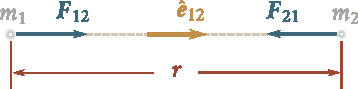
\includegraphics[scale=0.95]{figures/ch_06/fig_6_1.pdf}
			\caption[]{}
			\label{fig:6_1}
		\end{center}
	\end{minipage}
	\hspace{-0.05cm}
	\begin{minipage}[t]{0.5\linewidth}
		\begin{center}
			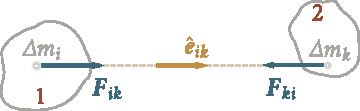
\includegraphics[scale=1]{figures/ch_06/fig_6_2.pdf}
			\caption[]{}
			\label{fig:6_2}
		\end{center}
	\end{minipage}
	\vspace{-0.3cm}
\end{figure}

In practice, the summation according to \eqn{6_5} consists in integration and, generally speaking, is a very complicated mathematical problem. If the interacting bodies are homogeneous and have a regular shape, the calculations are greatly simplified. In particular, when the interacting bodies are homogeneous\footnote{It is sufficient for the distribution of the mass within the limits of each sphere to have central symmetry, \ie, for the density to be a function only of the	distance from the centre of the sphere.} spheres, calculation by \eqn{6_5} leads to \eqn{6_2}, $m_1$ and $m_2$ now being the masses of the spheres, $r$ the distance between their centres, and $\vecuni{12}$ a unit vector directed from the centre of the first sphere to that of the second one. The spheres thus interact like point particles of masses equal to those of the spheres and situated at their centres.

If one of the bodies is a homogeneous sphere of a very great radius (for example, the Earth), while the second body can be considered as a point particle, then their interaction is described by \eqn{6_2} in which $r$ stands for the distance from the centre of the sphere to the particle (this statement will be proved in the following section).

The dimension of the gravitational constant in accordance with \eqn{6_1} is
\begin{equation*}
	[G] = \frac{[F][r^2]}{[m^2]} = \frac{(ML/T^2)L^2}{M^2} = L^3M^{-1}T^{-2}.
\end{equation*}

\noindent
The numerical value of $G$ was determined by measuring the force with which two bodies of known mass attract each other. Great difficulties appear in such measurements because the forces of attraction are extremely small for bodies whose masses can be measured directly. For example, two bodies each having a mass of \SI{100}{\kilo\gram} and one metre apart interact with a force of the order of \SI{e-6}{\newton}, \ie, about \SI{e-4}{\gf}.

\begin{figure}[t]
	\begin{center}
		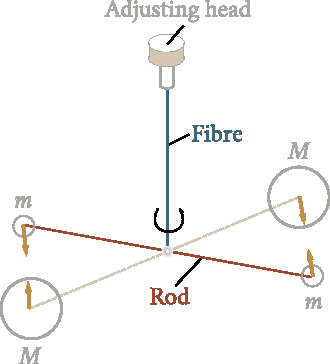
\includegraphics[scale=0.95]{figures/ch_06/fig_6_3.pdf}
		\caption[]{}
		\label{fig:6_3}
	\end{center}
\vspace{-0.7cm}
\end{figure}

The first successful attempt to determine $G$ was its measurement carried out by Henry Cavendish (1731-1810) in 1798. He used the very sensitive torsion balance method (\fig{6_3}). Two lead spheres $m$ (each of mass \SI{0.729}{\kilo\gram}) fastened to the ends of a light rod were placed near symmetrically arranged spheres $M$ (each of mass \SI{158}{\kilo\gram}). The rod was suspended on an elastic torsion fibre. Twisting of the latter was measured, and its magnitude showed the force of attraction between the spheres. The top end of the fibre was fastened in an adjusting head whose turning made it possible to change the distance between the spheres $m$ and $M$. The value
\begin{equation*}
	G = \SI{6.670e-11}{\metre\cubed\per\kilo\gram\per\second\squared}\,\,(\text{or}\,\, \si{\newton\metre\squared\per\kilo\gram\squared})
\end{equation*}

\noindent
is considered to be the most accurate of all the values determined in different ways.

If in \eqn{6_1} we assume that $m_1$, $m_2$, and $r$ equal unity, then the force numerically equals $G$. Thus, two spheres each having a mass of \SI{1}{\kilo\gram} whose centres are \SI{1}{\metre} apart attract each other with a force of \SI{6.670e-11}{\newton}.

\section{Gravitational Field}\label{sec:6_2}

Gravitational interaction is carried out through a gravitational field. Every body changes the properties of the space surrounding it---it sets up a gravitational field in this space. The field manifests itself in that another body placed in it experiences a force. The ``intensity'' of a gravitational field can obviously be assessed according to the magnitude of the force acting at a given point on a body of unit mass. Accordingly, the quantity
\begin{equation}\label{eq:6_6}
	\vec{g}' = \frac{\vec{F}}{m}
\end{equation}

\noindent
is called the \textbf{gravitational intensity}, or the \textbf{gravitational field vector}. In \eqn{6_6}, $\vec{F}$ is the gravitational force acting on a point particle of mass $m$ at a given point of the field.

The dimension of $\vec{g}'$ coincides with that of acceleration. The intensity of the gravitational field near the Earth's surface equals the acceleration of free fall $\vec{g}$ (with an accuracy up to the correction due to the Earth's rotation, see Sec.~\ref{sec:4_2}).

It is easy to conclude from \eqn{6_2} that the intensity of the field set up by a point particle of mass $m$ is
\begin{equation}\label{eq:6_7}
	\vec{g}' = -G\frac{m}{r^2}\vecuni{r}
\end{equation}

\noindent
where $\vecuni{r}$ is the unit vector of the position vector drawn from the particle to the given point of the field, and $r$ is the magnitude of this position vector.

Assume that a gravitational field is produced by a point particle of mass $m$ fixed at the origin of coordinates. Hence, the following force will act on a particle of mass $m'$ at a point with the position vector $\vec{r}$:
\begin{equation}\label{eq:6_8}
	\vec{F} = \vec{g}'m' = -G\frac{mm'}{r^2}\vecuni{r}
\end{equation}

\noindent
[compare with \eqn{3_120}]. We showed in Sec.~\ref{sec:3_13} that the potential energy of the particle $m'$ is determined in this case by the equation
\begin{equation}\label{eq:6_9}
	E_{\text{p}} = -G\frac{mm'}{r^2}
\end{equation}

\noindent
(the potential energy is assumed to vanish when $r\to\infty$). Equation~\eqref{eq:6_9} can also be interpreted as the mutual potential energy of the point particles $m$ and $m'$.

Inspection of \eqn{6_9} shows that to each point of the field produced by the particle $m$ there corresponds a definite value of the potential energy which the particle $m'$ has in this field. Consequently, the field can be characterized by the potential energy which a particle of mass $m'=1$ has at the given point. The quantity
\begin{equation}\label{eq:6_10}
	\varphi = \frac{E_{\text{p}}}{m'}
\end{equation}

\noindent
is called the \textbf{potential of the gravitational field}. In this equation, $E_{\text{p}}$ is the potential energy which a point particle of mass $m'$ has at a given point of the field.

Knowing the potential of a field, we can calculate the work done on the particle $m'$ by the forces of the field when moving it from position $1$ to position $2$. According to \eqn{3_30}, this work is
\begin{equation}\label{eq:6_11}
	A_{12} = E_{\text{p},1} - E_{\text{p},2} = m'(\varphi_1 - \varphi_2).
\end{equation}

According to Eqs.~\eqref{eq:6_6} and~\eqref{eq:6_10}, the force acting on the particle $m'$ is $\vec{F}=m'\vec{g}'$, and the potential energy of this particle is $E_{\text{p}}=m'\varphi$. By \eqn{3_31}, we have $\vec{F}=-\nabla E_{\text{p}}$, \ie, $m'\vec{g}'=-\nabla(m'\varphi)$. Putting the constant $m'$ outside the gradient sign and then cancelling this constant, we arrive at a relation between the intensity and potential of a gravitational field:
\begin{equation}\label{eq:6_12}
	\vec{g}' = -\nabla\varphi.
\end{equation}

\begin{figure}[t]
	\begin{center}
		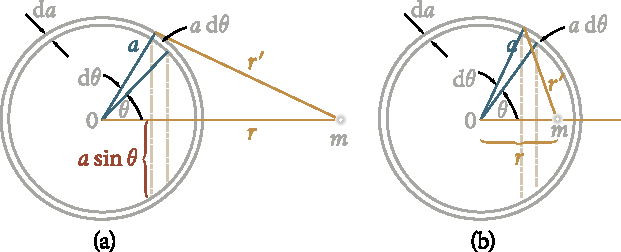
\includegraphics[scale=0.95]{figures/ch_06/fig_6_4.pdf}
		\caption[]{}
		\label{fig:6_4}
	\end{center}
	\vspace{-0.7cm}
\end{figure}

Let us find an expression for the mutual potential energy of a homogeneous spherical layer and a point particle of mass $m$. We shall consider two cases corresponding to the particle being outside and inside the layer, and shall begin with the former one (\fig{6_4}a). Let us separate from the layer a ring whose edges correspond to the values of the angle $\theta$ and $\theta+\deriv{\theta}$. The radius of this ring is $a\sin\theta$, and its width is a $\deriv{\theta}$ (here $a$ is the radius of the layer). Hence, the area of the ring is determined by the expression $2\pi a^2\sin\theta\,\deriv{\theta}$. If the thickness of the layer is $\deriv{a}$ and its density is $\rho$, then the mass of the ring is $2\pi\rho a^2\,\deriv{a}\,\sin\theta\,\deriv{\theta}$. All the points of the ring are at the same distance $r'$ from $m$. Consequently, by \eqn{6_9}, the mutual potential energy of the ring and the mass $m$ is determined by the expression
\begin{equation}\label{eq:6_13}
	\deriv{E_{\text{p}}} = -G\frac{2\pi\rho a^2\,\deriv{a}\,\sin\theta\,\deriv{\theta}\,m}{r'}.
\end{equation}

To obtain the potential energy of the entire spherical layer and the mass $m$, we must integrate \eqn{6_13} with respect to the angle $\theta$ within the limits from $0$ to $\pi$. Here the variable $r'$ varies within the limits from $r-a$ to $r+a$, where $r$ is the distance from the centre of the layer $0$ to $m$. Equation~\eqref{eq:6_13} contains two related variables, namely, $a$ and $r'$. We must exclude one of these variables prior to integration. The latter is simplified if we exclude the variable $\theta$. We can obtain the relation between $\theta$ and $r'$ by using the theorem of cosines. Inspection of \fig{6_4} shows that
\begin{equation*}
	r'^2 = a^2 + r^2 - 2ar\cos\theta.
\end{equation*}

\noindent
Differentiation of this expression yields
\begin{equation*}
	2r'\,\deriv{r'} = 2ar\sin\theta\,\deriv{\theta}.
\end{equation*}

\noindent
Hence, $\sin\theta\,\deriv{\theta}=(r'/ar)\,\deriv{r'}$. Making such a substitution in \eqn{6_13}, we get
\begin{equation*}
	\deriv{E_{\text{p}}} = -G\frac{2\pi\rho a\,\deriv{a}\,m\,\deriv{r'}}{r}.
\end{equation*}

\noindent
Integration with respect to $r'$ within the limits from $r_1'=r-a$ to $r_2'=r+a$ yields
\begin{equation}\label{eq:6_14}
	\deriv{E_{\text{p,lay}}} = -G\frac{2\pi\rho a\,\deriv{a}\,m}{r} \int_{r-a}^{r+a} \deriv{r'} = -G\frac{4\pi\rho a^2\,\deriv{a}\,m}{r}.
\end{equation}

\noindent
The expression $4\pi a^2\,\deriv{a}$ gives the volume of the layer, and $4\pi\rho a^2\,\deriv{a}$ its mass $\deriv{M}$. Thus, the mutual potential energy of the sphere layer and the mass $m$ is
\begin{equation}\label{eq:6_15}
	\deriv{E_{\text{p,lay}}} = -G\frac{\deriv{M}\,m}{r}
\end{equation}

\noindent
where $r$ is the distance from the centre of the layer to $m$.

All our calculations remain the same for the case when the mass is inside the layer (see \fig{6_4}b). Only the integration limits in \eqn{6_14} will differ because $r'$ changes in this case from $r_1'=r-a$ to $r_2'=r+a$. Consequently,
\begin{align}
	\deriv{E_{\text{p,lay}}'} &= -G\frac{2\pi\rho a\,\deriv{a}\,m}{r} \int_{a-r}^{a+r} \deriv{r'} = -G4\pi\rho a\,\deriv{a}\,m\nonumber\\
	& = -G \frac{4\pi\rho a^2\,\deriv{a}\,m}{a} = -G\frac{\deriv{M}\,m}{a}.\label{eq:6_16}
\end{align}

\noindent
Hence, in this case the potential energy is the same for all $r'$s and equals the value obtained in \eqn{6_15} for $r=a$.

Equation~\eqref{eq:6_15} can be interpreted as the potential energy of the particle $m$ in the field set up by a sphere layer of mass $\deriv{M}$. The derivative of this energy with respect to $r$ taken with the opposite sign equals the projection onto the direction $r$ of the force acting on the particle:
\begin{equation}\label{eq:6_17}
	\deriv{F_r} = -\diffpartial{E_{\text{p}}}{r} = -G\frac{\deriv{M}\,m}{r^2}.
\end{equation}

\noindent
The minus sign indicates that the force is directed toward the diminishing of $r$, \ie, to the centre of the layer.

It follows from \eqn{6_17} that the sphere layer acts on the particle with the same force that would be exerted on it by a point particle of a mass equal to that of the layer and placed at the centre of the latter.

Equation~\eqref{eq:6_16} does not depend on the coordinates of a particle. Therefore, the gradient of this function vanishes for all $r'$s less than $a$. Thus, no force acts on a particle inside the layer. Every element of the layer naturally exerts a certain force on the particle, but the sum of the forces exerted by all the elements of the layer equals zero.

Now let us consider a system consisting of a homogeneous sphere of mass $M$ and a point particle of mass $m$. Let us divide the sphere into layers of mass $\deriv{M}$. Each layer acts on the particle with a force determined by \eqn{6_17}. Summation of this expression over all the layers gives the force exerted on the particle by the sphere:
\begin{equation}\label{eq:6_18}
	F_r = \int\deriv{F_r} = -\int G\frac{\deriv{M}\,m}{r^2} = -G\frac{Mm}{r^2}.
\end{equation}

\noindent
The action of the sphere on the particle is equivalent to the action of a point particle of a mass equal to that of the sphere and placed at its centre (see the preceding section).

If we take a sphere with a spherical space inside, then no force will act on a particle in this space.

Summation of \eqn{6_15} over all the layers of a solid or a hollow sphere yields the mutual potential energy of a particle and a sphere:
\begin{equation}\label{eq:6_19}
	E_{\text{p}} = -G\frac{Mm}{r^2}.
\end{equation}

\noindent
Here $M$ is the mass of the sphere, $m$ is the mass of the particle, and $r$ is the distance from the particle to the centre of the sphere.

It follows from Eqs.~\eqref{eq:6_18} and~\eqref{eq:6_19} that the gravitational field produced by a homogeneous sphere is equivalent (outside the sphere) to the field produced by a point particle of the same mass at the centre of the sphere.

Let us consider two homogeneous spheres of masses $M_1$ and $M_2$. The second sphere experiences the same action on the part of the first one as would be exerted by a point particle of mass $M_1$ at the centre of the first sphere. According to Newton's third law, the corresponding force is equal in magnitude to the force that the second sphere would exert on the particle $M_1$. By \eqn{6_18}, the magnitude of this force is $GM_1M_2/r^2$. We have thus proved that homogeneous spheres interact like point particles at their centres.

\section{The Equivalence Principle}\label{sec:6_3}

Mass comes up in two different laws---in Newton's second law and in the law of universal gravitation. In the former case, it characterizes the inertial properties of bodies, and in the latter their gravitational properties, \ie, the ability of bodies to attract one another. In this connection, the question arises whether we ought to distinguish the inertial mass $m_{\text{in}}$ and the gravitational mass $m_{\text{g}}$.

This question can be answered only by experiments. Let us consider the free falling of bodies in a heliocentric reference frame. Any body near the Earth's surface experiences a force of attraction to the Earth that by \eqn{6_18} is
\begin{equation*}
	F = G\frac{m_{\text{g}} M_{\text{E}}}{R_{\text{E}}^2}
\end{equation*}

\noindent
where $m_{\text{g}}$ is the gravitational mass of a given body, $M_{\text{E}}$ is the gravitational mass of the Earth, and $R_{\text{E}}$ is the radius of the Earth.

This force causes the body to acquire the acceleration $a$ (but not $g$, see Sec.~\ref{sec:4_2}) that must equal the force $F$ divided by the inertial mass of the body $m_{\text{in}}$:
\begin{equation}\label{eq:6_20}
	a = \frac{F}{m_{\text{in}}} = G\frac{M_{\text{E}}}{R_{\text{E}}^2}\frac{m_{\text{g}}}{m_{\text{in}}}.
\end{equation}

Experiments show that the acceleration $a$ is the same for all bodies (it was shown in Sec.~\ref{sec:4_2} that the identical values of $a$ follow from the identical values of $g$). The factor $G(M_{\text{E}}/R_{\text{E}}^2)$ is also the same for all bodies. Consequently, the ratio $m_{\text{g}}/m_{\text{in}}$ is the same for all bodies too. All other experiments in which the difference between the inertial and the gravitational masses could manifest itself lead to a similar result.

We shall describe the experiment of R. E\"{o}tv\"{o}s, which he began in 1887 and continued over 25 years, as an example of such experiments. E\"{o}tv\"{o}s proceeded from the circumstance that a body at rest near the Earth's surface, apart from the reaction of its support, experiences the gravitational force $\vec{F}_{\text{g}}$ directed toward the Earth's centre and also the centrifugal force of inertia $\vec{F}_{\text{cf}}$ directed perpendicularly to the Earth's axis of rotation (\fig{6_5}---this figure is not drawn to scale---the magnitude of the centrifugal force is two orders smaller than that of the gravitational force, see Sec.~\ref{sec:4_2}). The gravitational force is proportional to the gravitational mass of a body $m_{\text{g}}$:
\begin{equation*}
	\vec{F}_{\text{g}} = m_{\text{g}}\vec{g}'
\end{equation*}

\noindent
($\vec{g}'$ is the gravitational intensity). The centrifugal force of inertia is proportional to the inertial mass $m_{\text{in}}$. According to \eqn{4_7}, its magnitude is determined by the expression
\begin{equation*}
	F_{\text{cf}} = m_{\text{in}}\omega^2R_{\text{E}}\cos\varphi
\end{equation*}

\noindent
where $\varphi$ is the latitude of the locality. It follows from \fig{6_5} that the magnitude of the vertical component of the centrifugal force of inertia is
\begin{equation*}
	F_{\text{vert}} = F_{\text{cf}}\cos\varphi =  m_{\text{in}}\omega^2R_{\text{E}}\cos^2\varphi = Am_{\text{in}}.
\end{equation*}

\noindent
We have introduced the symbol $A=\omega^2R_{\text{E}}\cos^2\varphi$. E\"{o}tv\"{o}s ran his experiment at the latitude of $\varphi=\SI{45}{\degree}$. In this case the coefficient $A$ is about one-hundredth of $g'$.

\begin{figure}[t]
	\begin{minipage}[t]{0.5\linewidth}
		\begin{center}
			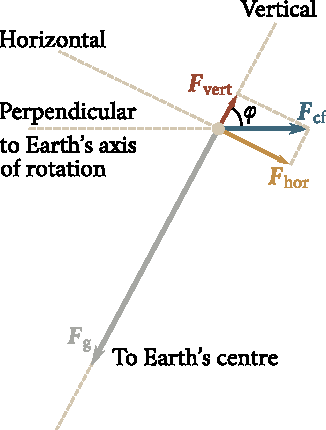
\includegraphics[scale=0.9]{figures/ch_06/fig_6_5.pdf}
			\caption[]{}
			\label{fig:6_5}
		\end{center}
	\end{minipage}
	\hspace{-0.05cm}
	\begin{minipage}[t]{0.5\linewidth}
		\begin{center}
			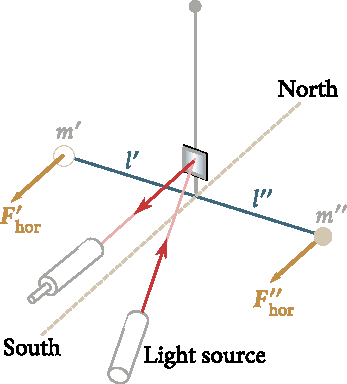
\includegraphics[scale=0.9]{figures/ch_06/fig_6_6.pdf}
			\caption[]{}
			\label{fig:6_6}
		\end{center}
	\end{minipage}
	\vspace{-0.5cm}
\end{figure}

The magnitude of the horizontal component of the force $F_{\text{cf}}$ is
\begin{equation*}
	F_{\text{hor}} = F_{\text{cf}}\sin\varphi =  m_{\text{in}}\omega^2R_{\text{E}}\cos\varphi\sin\varphi = Bm_{\text{in}}
\end{equation*}

\noindent
where $B=\omega^2R_{\text{E}}\cos\varphi\sin\varphi$ (for $\varphi=\SI{45}{\degree}$, the values of the coefficients A and B coincide).

E\"{o}tv\"{o}s suspended a rod with bodies fastened to its ends on an elastic thread (\fig{6_6}). The bodies were of different materials, but their masses were as equal as possible. A mirror was attached to the bottom part of the thread. The beam from the light source reflected from the mirror struck the cross hairs of a telescope. The arms $l'$ and $l''$ were selected so that the rod was in equilibrium in the vertical plane. The condition for this equilibrium is as follows:
\begin{equation}\label{eq:6_21}
	(m_{\text{g}}'g' - m_{\text{in}}'A)l' = (m_{\text{g}}''g' - m_{\text{in}}''A)l''.
\end{equation}

\noindent
The instrument was arranged with the rod perpendicular to the plane of the meridian (see \fig{6_6}). In this case, the horizontal components of the centrifugal force of inertia set up a twisting moment equal to
\begin{equation}\label{eq:6_22}
	M_{\text{t}} = m_{\text{in}}'Bl' - m_{\text{in}}''Bl''.
\end{equation}

\noindent
Eliminating the arm $l''$ from Eqs.~\eqref{eq:6_21} and~\eqref{eq:6_22}, we can arrive at the following equation after simple transformations:
\begin{equation*}
	M_{\text{t}} = m_{\text{in}}'Bl' \left[1 - \frac{(m_{\text{g}}'/m_{\text{in}}') g' - A}{(m_{\text{g}}''/m_{\text{in}}'') g' - A} \right].
\end{equation*}

\noindent
It can be seen from this equation that when the ratio of the gravitational and inertia masses is the same for both bodies, the moment twisting the thread must vanish. If the ratio $m_{\text{g}}/m_{\text{in}}$ for the first and second bodies is not the same, the twisting moment differs from zero. In this case when the entire instrument is turned through \SI{180}{\degree}, the twisting moment would reverse its sign and the light spot would move from the cross hairs of the telescope (\fig{6_7}). E\"{o}tv\"{o}s compared eight different bodies (including a wooden one) with a platinum body taken as the standard and discovered no twisting of the thread. This gave him the grounds to state that the ratio $m_{\text{g}}/m_{\text{in}}$ for these bodies is identical with an accuracy of \num{e-8}.

\begin{figure}[t]
	\begin{center}
		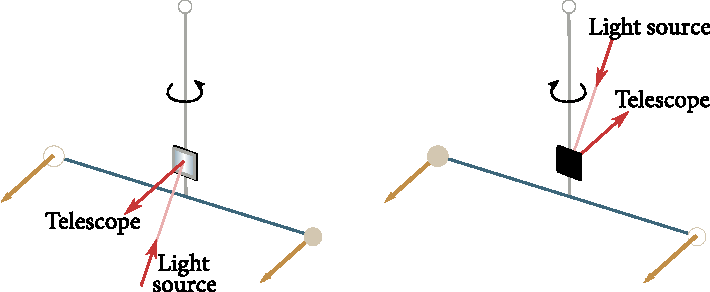
\includegraphics[scale=0.95]{figures/ch_06/fig_6_7.pdf}
		\caption[]{}
		\label{fig:6_7}
	\end{center}
	\vspace{-0.7cm}
\end{figure}

In 1961-1964, R. Dicke improved E\"{o}tv\"{o}s's method. He used the Sun's gravitational field and the centrifugal force of inertia due to the Earth's orbital motion for producing the twisting moment. As a result of his measurements, he arrived at the conclusion that the ratio $m_{\text{g}}/m_{\text{in}}$ is the same for the studied bodies with an accuracy of \num{e-11}. Finally, in 1971, V. Braginsky and V. Panov obtained the constancy of the ratio with an accuracy up to \num{e-12}.

Thus, all the experimental facts indicate that the inertial and gravitational masses of all bodies are strictly proportional to each other. This signifies that these masses become identical when the units are selected properly. This is why physicists simply speak of mass. Albert Einstein based his general theory of relativity on the gravitational and inertial masses being identical.

We have already noted in Sec.~\ref{sec:4_1} that the forces of inertia are similar to gravitational forces---both are proportional to the mass of the body which they are acting on. We have indicated there that if we are in a closed cab, no experiments will help us to establish what the action of the force $m\vec{g}$ is due to---whether it is due to the cab moving with the acceleration $-\vec{g}$, or to the fact that the stationary cab is near the Earth's surface. This statement forms the content of the so-called \textbf{equivalence principle}.

The identical nature of inertial and gravitational masses is the result of the equivalence of forces of inertia and gravitational forces.

It must be noted that from the very beginning we assumed in \eqn{6_1} that the mass coincides with the inertial mass of bodies, and we therefore determined the numerical value of $G$ assuming that $m_{\text{g}}/m_{\text{in}}$. We can thus write \eqn{6_20} in the form
\begin{equation}\label{eq:6_23}
	a = G\frac{M_{\text{E}}}{R_{\text{E}}^2}.
\end{equation}

\noindent
Equation~\eqref{eq:6_23} permits us to determine the mass of the Earth $M_{\text{E}}$. Use of the measured values of $a$, $R_{\text{E}}$ and $G$ in it gives the value of \SI{5.98e24}{\kilo\gram} for the Earth's mass.

Further, knowing the radius of the Earth's orbit $R_{\text{orb}}$ and the time $T$ of one complete revolution of the Earth about the Sun, we can find the Sun's mass $M_{\text{S}}$. The Earth's acceleration equal to $\omega^2R_{\text{orb}}$ (the angular velocity $\omega=2\pi/T$) is due to the force with which the Sun attracts the Earth. Hence,
\begin{equation*}
	M_{\text{E}}\omega^2R_{\text{orb}} = G\frac{M_{\text{E}}M_{\text{S}}}{R_{\text{orb}}^2}
\end{equation*}

\noindent
whence we can calculate the Sun's mass.

The masses of other celestial bodies were determined in a similar way.

\section{Orbital and Escape Velocities}\label{sec:6_4}

To travel about the Earth in a circular orbit with a radius differing only slightly from the Earth's radius $R_{\text{E}}$, a body must have a definite velocity $v_1$. Its value can be found from the condition of equality of the product of the mass of the body and its acceleration to the force of gravity acting on the body:
\begin{equation*}
	m\frac{m_1^2}{R_{\text{E}}} = mg.
\end{equation*}

\noindent
Hence,
\begin{equation}\label{eq:6_24}
	v_1 = (gR_{\text{E}})^{1/2}.
\end{equation}

Consequently, for a body to become a satellite of the Earth, it must be given the velocity $v_1$ called the \textbf{tangential} or \textbf{orbital velocity} ($v_1$ is also sometimes called the \textbf{first cosmic velocity}). Introduction of the values of $g$ and $R_{\text{E}}$ gives the following value for the orbital velocity:
\begin{equation*}
	v_1 = (gR_{\text{E}})^{1/2} = (9.8 \times 6.4 \times 10^6)^{1/2} \approx \SI{8e3}{\metre\per\second} = \SI{8}{\kilo\metre\per\second}.
\end{equation*}

A body having the velocity $v_1$ will not fall onto the Earth. This velocity, however, is not sufficient for the body to leave the sphere of the Earth's attraction, \ie, to travel away from the Earth over a distance such that its attraction to the Earth stops playing a significant part. The velocity $v_2$ required for this purpose is called the \textbf{escape velocity} (the \textbf{second cosmic velocity}).

To find the escape velocity, we must calculate the work that must be done against the forces of the Earth's attraction for moving a body from the Earth's surface to infinity. When a body moves away, the forces of the Earth's attraction do the following work on it:
\begin{equation*}
	A' = E_{\text{p,init}} - E_{\text{p,fin}}.
\end{equation*}

\noindent
According to \eqn{6_19}, the initial potential energy is
\begin{equation*}
	E_{\text{p,init}} = -G\frac{M_{\text{E}}m}{R_{\text{E}}}.
\end{equation*}

\noindent
and the final potential energy is zero. Thus,
\begin{equation*}
	A' = -G\frac{M_{\text{E}}m}{R_{\text{E}}}.
\end{equation*}

\noindent
The work $A$ that must be done against the forces of the Earth's attraction equals the work $A'$ taken with the opposite sign, \ie
\begin{equation}\label{eq:6_25}
	A = G\frac{M_{\text{E}}m}{R_{\text{E}}}.
\end{equation}

Disregarding the difference between the force of gravity $mg$ and the force of gravitational attraction of a body to the Earth, we can write that
\begin{equation*}
	mg = G\frac{M_{\text{E}}m}{R_{\text{E}}^2}.
\end{equation*}

\noindent
Hence,
\begin{equation*}
	G\frac{M_{\text{E}}m}{R_{\text{E}}} = mgR_{\text{E}}.
\end{equation*}

\noindent
Consequently, the work~\eqref{eq:6_25} can be written in the form
\begin{equation}\label{eq:6_26}
	A = mgR_{\text{E}}.
\end{equation}

A body leaving the Earth does this work at the expense of its store of kinetic energy. For this store of energy to be sufficient for doing the work~\eqref{eq:6_26}, the body must be projected from the Earth's surface with a velocity $v$ not lower than the value $v_2$ determined by the condition
\begin{equation*}
	\frac{mv_2^2}{2} = mgR_{\text{E}}
\end{equation*}

\noindent
whence
\begin{equation}\label{eq:6_27}
	v_2 = (2gR_{\text{E}})^{1/2}.
\end{equation}

\noindent
It is exactly the velocity $v_2$ that is the escape velocity from the Earth, or the second cosmic velocity. A comparison of Eqs.~\eqref{eq:6_27} and~\eqref{eq:6_24} shows that this velocity is $\sqrt{2}$ times greater than the orbital one. Multiplying \SI{8}{\kilo\metre\per\second} by $\sqrt{2}$, we get the approximate value of \SI{11}{\kilo\metre\per\second} by $v_2$.

It must be noted that the required magnitude of the velocity does not depend on the direction in which a body is launched from the Earth. This direction only affects the shape of the trajectory along which the body travels away from the Earth.

To leave the solar system, a body must overcome the forces of attraction to the Sun in addition to the Earth's attraction. The velocity of launching a body from the Earth's surface needed for this purpose is called the \textbf{escape velocity from the solar system}, the \textbf{space velocity}, or the \textbf{third cosmic velocity} $v_3$. The velocity $v_3$ depends on the direction of launching. When a body is launched in the direction of orbital motion of the Earth, this velocity is minimum and is about \SI{17}{\kilo\metre\per\second} (in this case the body's velocity relative to the Sun is the sum of its velocity relative to the Earth and the velocity with which the Earth is travelling about the Sun). When a body is launched in a direction opposite to that of the Earth's rotation, $v_3\approx \SI{73}{\kilo\metre\per\second}$.

The orbital and escape velocities were reached for the first time in the USSR. On October 4, 1957, the first successful launching of an artificial satellite of the Earth in the history of mankind was carried out in the Soviet Union. A second advance occurred on January 2, 1959. This day saw the launching from Soviet soil of a spaceship that escaped from the sphere of the Earth's attraction and became the first artificial planet of our solar system. On April 12, 1961, the first flight of a man into outer space was accomplished in the Soviet Union. The first Soviet cosmonaut Yuri Gagarin completed a flight around the Earth and landed successfully.
